\documentclass{article}

\usepackage[utf8]{inputenc}
\usepackage{caption}
\usepackage{subcaption}
\usepackage{natbib}
\usepackage{soul}
\usepackage{graphicx}
\usepackage{listings}
\usepackage[hyphens]{url}
\usepackage[table,xcdraw]{xcolor}
\usepackage{color}
\usepackage{textpos}
\usepackage{glossaries}
\usepackage{hyperref}
\usepackage{acronym}
\usepackage{verbatim}
\usepackage{amsmath}
\usepackage{amssymb}
\usepackage{comment}
\usepackage{xcolor}


\newcommand{\emailaddr}[1]{\href{mailto:#1}{\texttt{#1}}}

\begin{document}
\begin{titlepage}

  \newcommand{\HRule}{\rule{\linewidth}{0.5mm}}
  \center
  
  \textsc{\Large Department of Computer Science And Engineering}\\[0.5cm]
  
  \textsc{\Large University of Bologna}\\[0.6cm]
  
  \hrule width \hsize \kern 1mm \hrule width \hsize height 2pt 
  \vspace{0.8cm}
  { \large \bfseries DealerPro}\\[0.6cm]
  { \large \bfseries Risk Analysis}\\[0.6cm]
  { \large Project Management}\\[0.6cm]
  
  
  {\bfseries{June, 2023}
  \hfill
  \bfseries{Davide Domini}}\\[0.6cm]
  
  \hrule width \hsize height 2pt \kern 1mm \hrule width \hsize height 1pt
  \vspace{0.4cm}
  
  \end{titlepage}

  \clearpage
  
  \section{Matrice dei rischi}

  \begin{figure}[h!]
    \centering
    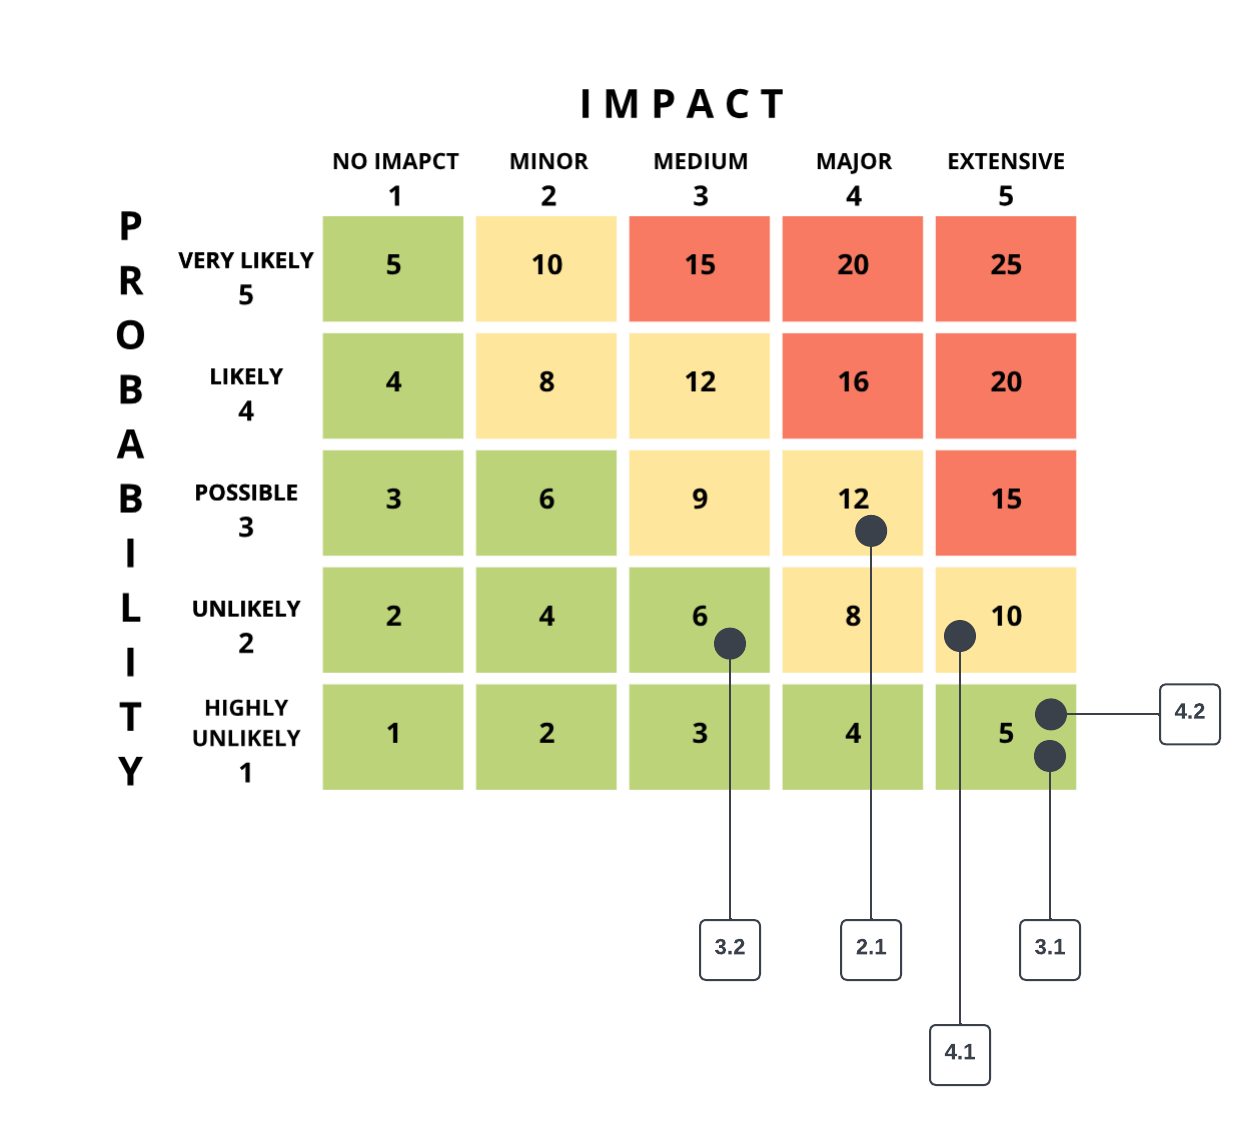
\includegraphics[width=\textwidth]{imgs/riskmatrix.png}
    \caption{Matrice dei rischi}
    \label{fig:risk_matrix}
  \end{figure}

  \section{Rischi tecnici}

  \subsection{Complessità cloud}
  \begin{itemize}
    \item \textbf{Probabilità}: Medium (3)
    \item \textbf{Conseguenze}: Major (4)
    \item \textbf{Score}: 12
    \item \textbf{Descrizione}: Lo sviluppo di un'architettura a micro-servizi complessa sfruttando
        soluzioni cloud potrebbe portare a ritardi e violazioni del budget a causa di una
        errata e complessa configurazione del sistema cloud.
  \end{itemize}


  \section{Rischi di organizzazione}
  \subsection{Mancanza di risorse umane}
  \begin{itemize}
    \item \textbf{Probabilità}: Highly unlikely (1)
    \item \textbf{Conseguenze}: Extensive (5)
    \item \textbf{Score}: 5
    \item \textbf{Descrizione}: La mancanza di risorse umane sarebbe un problema molto 
        grave che potrebbe portare a ritardi consistenti, tuttavia è molto improbabile 
        che accada.
  \end{itemize}

  \subsection{Mancanza di budget}
  \begin{itemize}
    \item \textbf{Probabilità}: Unlikely (2)
    \item \textbf{Conseguenze}: Medium (3)
    \item \textbf{Score}: 6
    \item \textbf{Descrizione}: La mancanza di budget potrebbe portare a ritardi e 
        a una riduzione della qualità del prodotto.
  \end{itemize}

  \section{Rischi di gestione del progetto}

  \subsection{Complessità integrazione sottoprogetti}
  \begin{itemize}
    \item \textbf{Probabilità}: Unlikely (2)
    \item \textbf{Conseguenze}: Extensive (5)
    \item \textbf{Score}: 10
    \item \textbf{Descrizione}: Una non adeguata gestione dei sotto-progetti 
        può portare a problematiche nelle fasi di integrazione tra le varie unità.
  \end{itemize}

  \subsection{Peggiorare i processi aziendali del committente}
  \begin{itemize}
    \item \textbf{Probabilità}: Higly unlikely (1)
    \item \textbf{Conseguenze}: Extensive (5)
    \item \textbf{Score}: 5
    \item \textbf{Descrizione}: Un testig non adeguato del sistema potrebbe introdurre bug 
        che andrebbero a peggiorare i processi aziendali del committente.
  \end{itemize}


\end{document}
